\chapter{Geodésicas, aceleración uniforme y límite newtoniano}

El problema inmediato es la gravedad. Más precisamente, queremos encontrar la métrica del espacio-tiempo que describe un campo gravitatorio casi uniforme, como el campo de un pequeño laboratorio cerca de la superficie terrestre. Resulta que la vía más corta para obtener esa métrica no es directa. Primero debemos dar un significado operativo a tres ideas geométricas: la derivación covariante, el transporte paralelo y el movimiento geodésico.

Estas ideas dependen unas de otras. La derivación covariante indica cómo comparar vectores en puntos vecinos. El transporte paralelo indica cómo desplazar un vector sin girarlo. Una geodésica se obtiene cuando el vector transportado es la tangente a la propia trayectoria. Cuando la trayectoria se encuentra en el espacio-tiempo y no en el espacio, esa misma ecuación geodésica se convierte en la ecuación de movimiento de una partícula en caída libre.

En la segunda mitad de la clase se da entonces un paso sorprendente. Seguimos en el espacio-tiempo plano de Minkowski, pero lo describimos con coordenadas adaptadas a una familia rígida de observadores acelerados. En esas coordenadas, la métrica parece gravitatoria. Cerca de un observador reproduce el potencial de un campo uniforme, y sus geodésicas obedecen la ecuación newtoniana
\begin{equation}
\frac{d^2y}{d\tau^2}=-g.
\end{equation}
Este es el principio de equivalencia expresado mediante un cálculo.

\section{Repaso de la derivada covariante}

En un punto elegido \(P\), se pueden escoger coordenadas lo más cartesianas posible. Al principio, la clase las llama coordenadas normales de Gauss y enseguida matiza ese nombre. Lo importante son las condiciones locales:
\begin{equation}
g_{mn}(P)=\delta_{mn},
\qquad
\partial_r g_{mn}(P)=0.
\label{eq:l4-normal-point}
\end{equation}
Son coordenadas normales en un punto. No tienen por qué seguir siendo cartesianas en un entorno finito, y existen muchos marcos de este tipo porque sus ejes se pueden girar.

La métrica es compatible con el operador derivada:
\begin{equation}
\nabla_r g_{mn}=0,
\qquad
\nabla_r g^{mn}=0.
\label{eq:l4-metric-compatibility}
\end{equation}
Para un covector \(V_s\), la derivada covariante es
\begin{equation}
\nabla_r V_s
=
\partial_r V_s-\Gamma^p{}_{rs}V_p.
\label{eq:l4-covector-derivative}
\end{equation}
Los coeficientes de conexión son
\begin{equation}
\Gamma^p{}_{rs}
=
\frac{1}{2}g^{pn}
\left(
\partial_s g_{nr}
+\partial_r g_{ns}
-\partial_n g_{rs}
\right).
\label{eq:l4-christoffel}
\end{equation}
Al escribir esta expresión en la pizarra, se corrigen varios índices. La ecuación \eqref{eq:l4-christoffel} es la relación completa. Es simétrica en \(r\) y \(s\), como corresponde a la conexión de Levi-Civita sin torsión.

\begin{figure}[htbp]
\centering
\includegraphics[width=0.92\textwidth]{lecture_04_figure_01.png}
\caption{La derivada de un covector y la fórmula completa de los símbolos de Christoffel.}
\end{figure}

Como los símbolos de Christoffel se construyen a partir de las primeras derivadas de la métrica, se anulan en \(P\) en las coordenadas \eqref{eq:l4-normal-point}. No se anulan en todos los sistemas de coordenadas, ni siquiera cuando el espacio subyacente es plano. Por tanto, \(\Gamma^p{}_{rs}\) no es un tensor. Más adelante, ese carácter no tensorial será precisamente lo que permita a un observador acelerado describir una fuerza gravitatoria que un observador inercial no percibe.

\subsection{Subir el índice del vector}

La derivada correspondiente de un vector no se introduce como una regla aparte que haya que memorizar. Se deduce de la métrica. Empezamos con
\begin{equation}
V^n=g^{np}V_p.
\end{equation}
Entonces
\begin{align}
\nabla_m V^n
&=\nabla_m\!\left(g^{np}V_p\right) \\
&=(\nabla_m g^{np})V_p+g^{np}\nabla_m V_p \\
&=g^{np}\left(\partial_mV_p-\Gamma^r{}_{mp}V_r\right),
\end{align}
donde la compatibilidad métrica elimina el primer término. Al reordenar los índices se obtiene
\begin{equation}
\nabla_m V^n
=
\partial_m V^n+\Gamma^n{}_{mr}V^r.
\label{eq:l4-vector-derivative}
\end{equation}

\begin{figure}[htbp]
\centering
\includegraphics[width=0.90\textwidth]{lecture_04_figure_02.png}
\caption{Subir el índice con la métrica inversa antes de derivar.}
\end{figure}

\begin{figure}[htbp]
\centering
\includegraphics[width=0.90\textwidth]{lecture_04_figure_03.png}
\caption{La derivada con índice superior que se obtiene de la compatibilidad métrica y la regla del producto.}
\end{figure}

La regla de los índices es, por tanto, sencilla:
\begin{equation}
\boxed{
\begin{aligned}
\text{lower index:}&\quad -\Gamma,\\
\text{upper index:}&\quad +\Gamma.
\end{aligned}}
\end{equation}
Para un tensor de rango superior aparece un término de conexión por cada índice, y el signo depende de si ese índice es inferior o superior.

\subsection{Una pregunta terminológica}

¿Cuáles son exactamente las mejores coordenadas mencionadas antes? No se afirma que constituyan un sistema de coordenadas global privilegiado. En un punto elegido, hacen que la métrica adopte su forma plana y que sus primeras derivadas se anulen. Si se giran los ejes, se obtiene otro marco igual de válido. Las afirmaciones geométricas deducidas en ese marco no dependen de su orientación, porque los objetos finales son tensores.

\section{Transporte paralelo a lo largo de una curva}

Supongamos que un vector \(V^n\) se transporta a lo largo de una curva. Durante un desplazamiento infinitesimal \(dx^m\), su variación covariante es
\begin{align}
\delta V^n
&=(\nabla_mV^n)\,dx^m \\
&=\partial_mV^n\,dx^m
+\Gamma^n{}_{mr}V^r\,dx^m \\
&=dV^n+\Gamma^n{}_{mr}V^r\,dx^m.
\label{eq:l4-covariant-differential}
\end{align}

\begin{figure}[htbp]
\centering
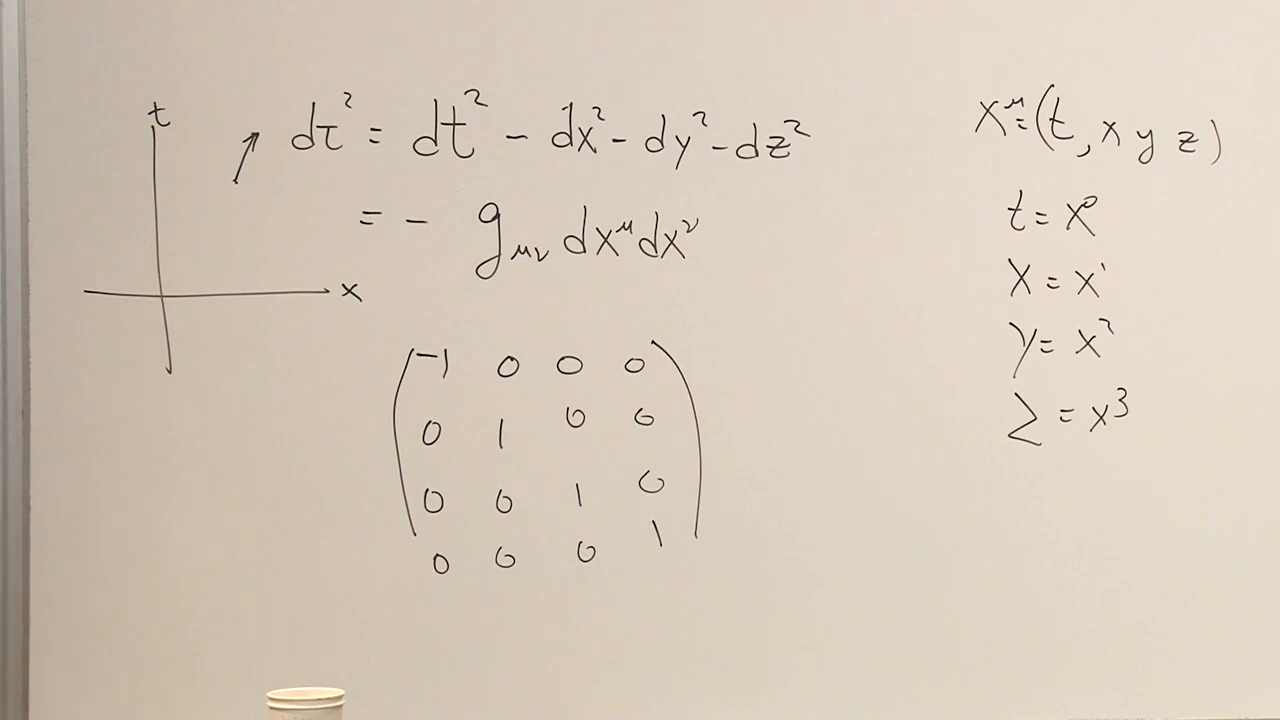
\includegraphics[width=0.92\textwidth]{lecture_04_figure_04.png}
\caption{La variación ordinaria de las componentes y la corrección de conexión a lo largo de una curva.}
\end{figure}

El vector se transporta en paralelo cuando esta variación covariante se anula:
\begin{equation}
\boxed{
dV^n+\Gamma^n{}_{mr}V^r\,dx^m=0.
}
\label{eq:l4-parallel-transport}
\end{equation}
Operativamente, podemos imaginar que construimos un marco normal en cada punto de la curva. En ese marco local, se exige que el vector transportado no gire. Luego avanzamos una distancia infinitesimal, construimos el siguiente marco normal y repetimos el procedimiento.

\begin{figure}[htbp]
\centering
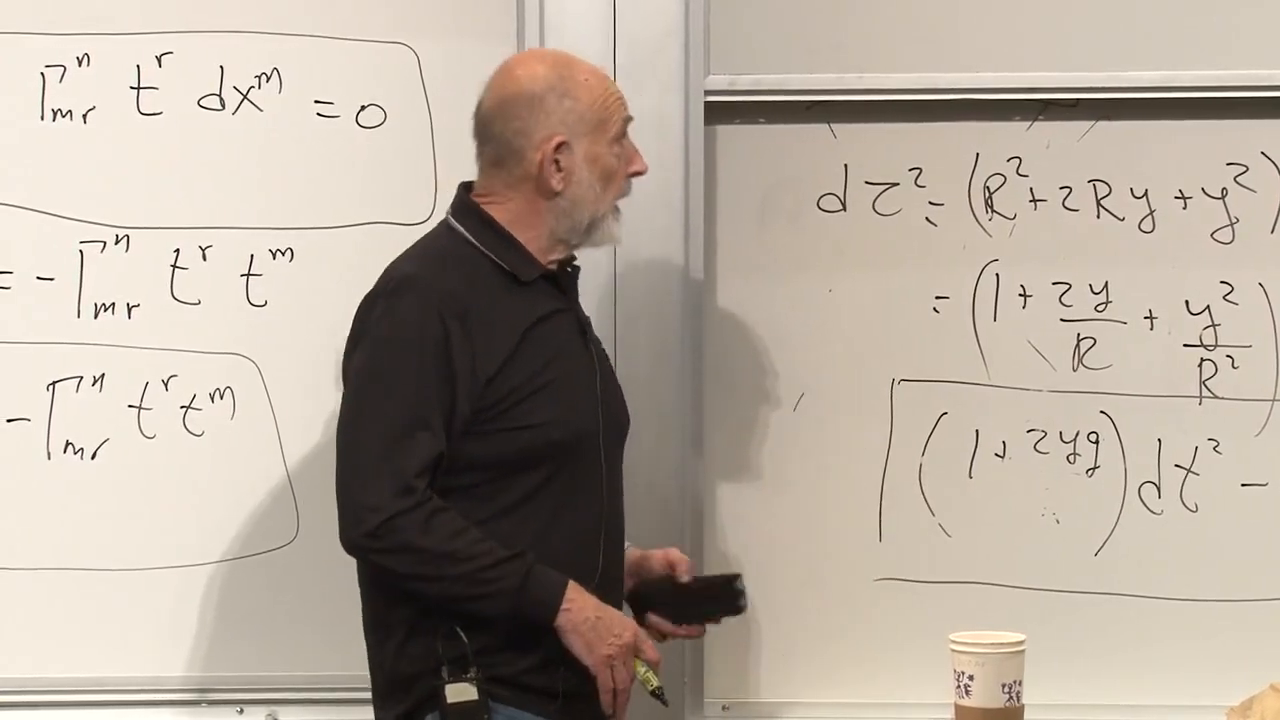
\includegraphics[width=0.92\textwidth]{lecture_04_figure_05.png}
\caption{Una versión clara en la pizarra de la ecuación de transporte paralelo.}
\end{figure}

La orientación de cada marco normal provisional no forma parte de la física. Podríamos girarlo antes de hacer la comparación. Lo importante es que la afirmación covariante \eqref{eq:l4-parallel-transport} no dependa de esa elección arbitraria.

\subsection{Dependencia de la trayectoria y curvatura}

En un espacio curvo, el transporte paralelo depende de la trayectoria. Partamos del mismo vector en el mismo punto inicial y transportémoslo hasta el mismo punto final por dos caminos distintos. En general, los vectores finales serán diferentes. Al transportar un vector alrededor de un lazo cerrado, este puede regresar girado. Esa discrepancia es la holonomía y constituye una señal directa de curvatura.

\begin{figure}[htbp]
\centering
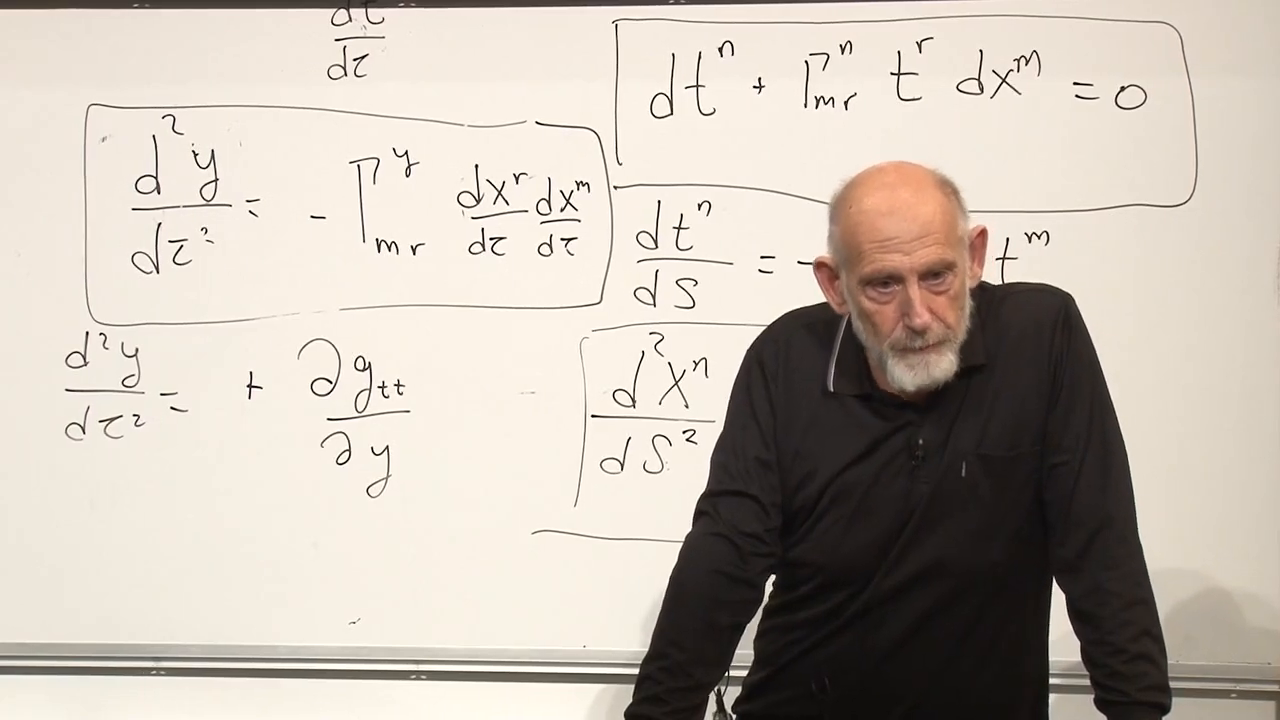
\includegraphics[width=0.90\textwidth]{lecture_04_figure_06.png}
\caption{En una superficie curva, dos trayectorias pueden transportar un vector hasta orientaciones finales distintas.}
\end{figure}

El cono ofrece un ejemplo útil. Lejos del vértice, se puede cortar un cono y extenderlo en el plano. Sin embargo, el transporte paralelo alrededor de un lazo que rodea el vértice devuelve el vector girado en un ángulo igual al déficit angular. Si se redondea el vértice, la curvatura es finita y se distribuye en una región pequeña. Si es perfectamente agudo, la idealización concentra la curvatura en el vértice.

\begin{figure}[htbp]
\centering
\includegraphics[width=0.90\textwidth]{lecture_04_figure_07.png}
\caption{Movimiento circular sobre el cono y su representación plana al desplegarlo.}
\end{figure}

\subsection{Preguntas sobre el vector transportado}

\paragraph{¿Tiene que estar definido el vector en todas partes?}
No. Se puede partir de un solo vector en un punto y resolver \eqref{eq:l4-parallel-transport} únicamente a lo largo de la curva elegida. No es necesario definir un campo vectorial completo. Si se ha definido un campo en una región, puede ser covariantemente constante en una dirección y no serlo en otra.

\paragraph{¿Se conserva su longitud?}
Sí. Sea \(V^2=g_{mn}V^mV^n\). A lo largo de la curva,
\begin{align}
\frac{D}{d\lambda}\left(g_{mn}V^mV^n\right)
&=
\frac{Dg_{mn}}{d\lambda}V^mV^n
+2g_{mn}V^m\frac{DV^n}{d\lambda}\\
&=0.
\end{align}
La compatibilidad métrica hace que el primer término se anule, y el transporte paralelo hace que se anule el segundo. Por tanto, se conservan las longitudes y los ángulos mutuos de los vectores transportados en paralelo.

\paragraph{¿Se transporta en paralelo la tangente a cualquier curva?}
No. Esta pregunta conduce directamente a las geodésicas. La tangente a una trayectoria circular alrededor de un cono cambia continuamente de dirección. La tangente a la recta que se obtiene al desplegar el cono no lo hace. Solo la segunda trayectoria es localmente recta.

\section{Geodésicas: las trayectorias más rectas, no simplemente las más cortas}

Una geodésica admite dos descripciones relacionadas. Globalmente, es una trayectoria estacionaria del funcional de longitud o de tiempo propio. Localmente, es la trayectoria más recta posible. La palabra estacionaria es importante: según la geometría y los extremos, la trayectoria no tiene por qué ser el único mínimo global. En el espacio-tiempo lorentziano, las geodésicas temporales maximizan localmente el tiempo propio, en vez de minimizar una distancia positiva.

Aquí necesitamos la descripción local. Un automóvil pequeño que avanza por un terreno curvo con el volante fijo en la posición de marcha recta describe una geodésica, siempre que sea pequeño en comparación con la escala en que se curva el terreno. Puede que no parezca recto en un espacio de inmersión; es recto según la geometría disponible sobre la superficie.

\begin{figure}[htbp]
\centering
\includegraphics[width=0.90\textwidth]{lecture_04_figure_08.png}
\caption{Una trayectoria trazada intrínsecamente sobre la superficie curva, como preparación para definir la trayectoria más recta.}
\end{figure}

\subsection{El vector tangente}

Sea la curva \(x^m(s)\), con longitud de arco
\begin{equation}
ds^2=g_{mn}\,dx^m dx^n.
\end{equation}
El vector tangente unitario es
\begin{equation}
t^m=\frac{dx^m}{ds}.
\label{eq:l4-unit-tangent}
\end{equation}
Geométricamente, tomamos dos puntos cercanos, formamos el vector desplazamiento entre ellos, lo dividimos por la distancia que los separa y hacemos que los puntos se aproximen hasta coincidir.

\begin{figure}[htbp]
\centering
\includegraphics[width=0.90\textwidth]{lecture_04_figure_09.png}
\caption{La dirección tangente como límite del desplazamiento a lo largo de una curva.}
\end{figure}

\begin{figure}[htbp]
\centering
\includegraphics[width=0.90\textwidth]{lecture_04_figure_10.png}
\caption{El elemento de línea y el vector tangente unitario \(t^m=dx^m/ds\).}
\end{figure}

Una geodésica es una curva cuya tangente se transporta en paralelo a lo largo de ella misma:
\begin{equation}
dt^n+\Gamma^n{}_{mr}t^r\,dx^m=0.
\end{equation}
Dividimos por \(ds\) y usamos \(dx^m/ds=t^m\):
\begin{equation}
\frac{dt^n}{ds}
=
-\Gamma^n{}_{mr}t^m t^r.
\end{equation}
Por último, sustituimos \(t^n=dx^n/ds\):
\begin{equation}
\boxed{
\frac{d^2x^n}{ds^2}
+\Gamma^n{}_{mr}
\frac{dx^m}{ds}
\frac{dx^r}{ds}
=0.
}
\label{eq:l4-geodesic}
\end{equation}

\begin{figure}[htbp]
\centering
\includegraphics[width=0.94\textwidth]{lecture_04_figure_11.png}
\caption{La ley de transporte del vector tangente y la ecuación geodésica de segundo orden.}
\end{figure}

La ecuación \eqref{eq:l4-geodesic} ya se parece a la dinámica newtoniana. Si se sustituye \(s\) por un parámetro temporal apropiado, el primer término es una aceleración. El término de conexión actúa entonces como una fuerza por unidad de masa, determinada enteramente por la métrica. En relatividad general, la analogía se vuelve literal: las partículas libres siguen geodésicas del espacio-tiempo, y lo que Newton llamaba aceleración gravitatoria aparece a través de la conexión.

\section{De la distancia riemanniana al tiempo propio del espacio-tiempo}

La exposición pasa ahora del espacio curvo al espacio-tiempo. En coordenadas cartesianas inerciales, el tiempo propio entre sucesos cercanos es
\begin{equation}
d\tau^2
=dt^2-dx^2-dy^2-dz^2.
\label{eq:l4-proper-time}
\end{equation}
La clase usa
\begin{equation}
d\tau^2=-g_{\mu\nu}\,dx^\mu dx^\nu
\label{eq:l4-lecture-sign}
\end{equation}
con
\begin{equation}
g_{\mu\nu}
=
\eta_{\mu\nu}
=
\begin{pmatrix}
-1&0&0&0\\
0&1&0&0\\
0&0&1&0\\
0&0&0&1
\end{pmatrix}.
\label{eq:l4-eta}
\end{equation}
Así, el signo menos externo de \eqref{eq:l4-lecture-sign} convierte la métrica elegida, de signatura mayormente positiva, en \eqref{eq:l4-proper-time}. Las coordenadas son
\begin{equation}
\begin{aligned}
x^\mu&=(t,x,y,z),\\
x^0&=t,\quad x^1=x,\\
x^2&=y,\quad x^3=z.
\end{aligned}
\end{equation}

\begin{figure}[htbp]
\centering
\includegraphics[width=0.94\textwidth]{lecture_04_figure_12.png}
\caption{El tiempo propio, las coordenadas del espacio-tiempo y la métrica de Minkowski de signatura mayormente positiva.}
\end{figure}

La signatura contiene la información invariante: un valor propio tiene el signo asociado al tiempo y tres tienen el signo asociado al espacio. Multiplicar toda la métrica por \(-1\) y ajustar coherentemente todas las convenciones da la convención, también muy habitual, de signatura mayormente negativa. Ningún aspecto físico depende de esa elección global.

La clase pregunta si se han considerado espacios con otras signaturas indefinidas. Matemáticamente, las geometrías seudoriemannianas con muchas signaturas están bien establecidas. La cuestión física es más acotada: el espacio-tiempo relativista observado es lorentziano, con una dirección temporal. Direcciones temporales adicionales alterarían profundamente la estructura causal y no describen la física que estamos estudiando.

\begin{figure}[htbp]
\centering
\includegraphics[width=0.94\textwidth]{lecture_04_figure_13.png}
\caption{Se comprueba la convención de signos antes de denotar la métrica plana por \(\eta_{\mu\nu}\).}
\end{figure}

Que el espacio-tiempo sea plano no significa que las componentes de la métrica deban tener la forma \(\eta_{\mu\nu}\) en todo sistema de coordenadas. Significa que existe algún sistema en el que sí la tienen. Las coordenadas curvilíneas o aceleradas pueden hacer que las componentes varíen con la posición aunque el tensor de Riemann sea nulo.

\section{Por qué una aceleración coordenada igual no produce rigidez}

Queremos construir coordenadas ligadas a un ascensor acelerado. La primera idea es alinear varios observadores separados por distancias fijas y asignarles a todos la misma aceleración coordenada. La relatividad impide que esa construcción ingenua siga siendo rígida.

\begin{figure}[htbp]
\centering
\includegraphics[width=0.92\textwidth]{lecture_04_figure_14.png}
\caption{Una fila de observadores vecinos permite comprobar si una aceleración común conserva la rigidez.}
\end{figure}

Si, según un mismo marco inercial, observadores separados siguen programas de aceleración idénticos, la distancia entre ellos en sus marcos de reposo instantáneos cambiantes no permanece constante. Una cuerda que los une se estira y acaba rompiéndose. Es la misma tensión cinemática que se manifiesta en el experimento mental de las naves de Bell. Además, una aceleración coordenada newtoniana constante no puede mantenerse indefinidamente: acabaría prediciendo una velocidad superior a la de la luz.

Por tanto, un marco acelerado rígido relativista debe tener una aceleración propia distinta en cada posición. Los observadores más próximos al horizonte que se formaría aceleran más; los más alejados aceleran menos. Así, sus separaciones propias pueden permanecer constantes en el marco comóvil instantáneo. Esto es una aceleración rígida en el sentido de Born en una dimensión espacial.

\section{Coordenadas polares euclidianas como preparación}

La construcción correcta se aprecia mejor si empezamos por un círculo ordinario. En un plano euclidiano,
\begin{equation}
x=r\cos\theta,
\qquad
y=r\sin\theta,
\end{equation}
de modo que
\begin{equation}
x^2+y^2=r^2,
\qquad
\cos^2\theta+\sin^2\theta=1.
\end{equation}
Las expresiones con exponenciales complejas son
\begin{equation}
\cos\theta=\frac{e^{i\theta}+e^{-i\theta}}{2},
\qquad
\sin\theta=\frac{e^{i\theta}-e^{-i\theta}}{2i}.
\label{eq:l4-euler-trig}
\end{equation}
Durante la discusión en la pizarra se detecta y restituye el factor \(i\) que falta en el denominador de la fórmula del seno.

\begin{figure}[htbp]
\centering
\includegraphics[width=0.94\textwidth]{lecture_04_figure_15.png}
\caption{El círculo, las coordenadas polares euclidianas y sus expresiones trigonométricas exponenciales.}
\end{figure}

Un valor fijo de \(r\) corresponde a un círculo. El movimiento con velocidad angular constante tiene aceleración centrípeta de módulo constante, siempre dirigida hacia dentro. En el espacio-tiempo, la hipérbola desempeñará el papel correspondiente.

\section{Coordenadas hiperbólicas en el espacio-tiempo de Minkowski}

Sustituyamos las funciones trigonométricas por sus análogas hiperbólicas:
\begin{equation}
\cosh\omega=\frac{e^\omega+e^{-\omega}}{2},
\qquad
\sinh\omega=\frac{e^\omega-e^{-\omega}}{2},
\end{equation}
con
\begin{equation}
\cosh^2\omega-\sinh^2\omega=1.
\label{eq:l4-hyperbolic-identity}
\end{equation}
No aparece ningún factor \(i\). La coordenada \(\omega\) es un ángulo hiperbólico, o rapidez. A diferencia de un ángulo ordinario, no es periódica; varía entre \(-\infty\) y \(+\infty\).

\begin{figure}[htbp]
\centering
\includegraphics[width=0.94\textwidth]{lecture_04_figure_16.png}
\caption{En la construcción del espacio-tiempo, las funciones hiperbólicas sustituyen a las funciones circulares.}
\end{figure}

Definamos nuevas coordenadas en la cuña derecha de Rindler:
\begin{equation}
x=r\cosh\omega,
\qquad
t=r\sinh\omega,
\qquad
r>0.
\label{eq:l4-rindler-transform}
\end{equation}
Entonces
\begin{equation}
x^2-t^2=r^2.
\label{eq:l4-rindler-hyperbola}
\end{equation}
A \(r\) fijo, la variación de \(\omega\) traza una hipérbola. Al aumentar \(r\), se avanza a través de la familia en una dirección espacial; al aumentar \(\omega\), se avanza a lo largo de una hipérbola en una dirección temporal.

\begin{figure}[htbp]
\centering
\includegraphics[width=0.94\textwidth]{lecture_04_figure_17.png}
\caption{La transformación de coordenadas \(x=r\cosh\omega\), \(t=r\sinh\omega\) y su hipérbola invariante.}
\end{figure}

\begin{figure}[htbp]
\centering
\includegraphics[width=0.94\textwidth]{lecture_04_figure_18.png}
\caption{Una congruencia de hipérbolas con \(r\) fijo que representa una familia rígidamente acelerada.}
\end{figure}

\subsection{La métrica en coordenadas aceleradas}

Derivemos \eqref{eq:l4-rindler-transform}:
\begin{align}
dx&=\cosh\omega\,dr+r\sinh\omega\,d\omega,\\
dt&=\sinh\omega\,dr+r\cosh\omega\,d\omega.
\end{align}
Al usar \eqref{eq:l4-hyperbolic-identity}, los términos cruzados se cancelan:
\begin{align}
d\tau^2
&=dt^2-dx^2\\
&=r^2\,d\omega^2-dr^2.
\label{eq:l4-rindler-metric}
\end{align}
Al recuperar las direcciones transversales, simplemente se añade \(-dy^2-dz^2\) a la convención de tiempo propio usada aquí.

Seguimos teniendo espacio-tiempo plano. El coeficiente dependiente de las coordenadas \(r^2\) no es más indicio de curvatura que el factor \(r^2\) que multiplica a \(d\theta^2\) en las coordenadas polares euclidianas.

\subsection{Aceleración propia a lo largo de las hipérbolas}

Para una línea de universo fija \(r=R\), la ecuación \eqref{eq:l4-rindler-metric} da
\begin{equation}
d\tau=R\,d\omega.
\end{equation}
Su cuadrivelocidad es
\begin{equation}
U^\mu
=
\frac{d(t,x)}{d\tau}
=
(\cosh\omega,\sinh\omega),
\end{equation}
y su cuadraceleración es
\begin{equation}
A^\mu
=
\frac{dU^\mu}{d\tau}
=
\frac{1}{R}(\sinh\omega,\cosh\omega).
\end{equation}
El módulo invariante es constante:
\begin{equation}
a=\sqrt{A^\mu A_\mu}=\frac{1}{R}
\qquad (c=1).
\label{eq:l4-proper-acceleration}
\end{equation}

\begin{figure}[htbp]
\centering
\includegraphics[width=0.90\textwidth]{lecture_04_figure_19.png}
\caption{La ley de proporcionalidad inversa al radio \(a=1/R\) para una línea de universo acelerada fija.}
\end{figure}

Al restituir las unidades,
\begin{equation}
\boxed{a=\frac{c^2}{R}.}
\label{eq:l4-proper-acceleration-units}
\end{equation}

\begin{figure}[htbp]
\centering
\includegraphics[width=0.90\textwidth]{lecture_04_figure_20.png}
\caption{Al restituir las unidades, \(1/R\) se convierte en \(c^2/R\).}
\end{figure}

Cuanto menor es la intersección \(R\), más pronunciada es la curvatura de la línea de universo y mayor es la aceleración propia que siente su observador. Las hipérbolas más alejadas se curvan menos y requieren menos aceleración. Cada observador tiene una aceleración constante en el tiempo, pero las aceleraciones de observadores distintos son diferentes. Esa variación es precisamente lo que conserva sus distancias propias mutuas.

\subsection{Preguntas sobre las coordenadas aceleradas}

\paragraph{¿Es \(R\) la intersección con el eje \(x\)?}
Sí. Para \(\omega=0\), la ecuación \eqref{eq:l4-rindler-transform} da \(t=0\) y \(x=R\). La intersección determina la aceleración propia mediante \eqref{eq:l4-proper-acceleration-units}.

\paragraph{¿Depende la construcción del origen elegido?}
Las coordenadas sí dependen de él. Trasladar el origen produce otra familia de hipérbolas con asíntotas desplazadas. Ninguna física invariante depende de esa elección. Seleccionamos deliberadamente un sistema de coordenadas acelerado y preguntamos cómo se describe en él el movimiento inercial.

\paragraph{¿Qué es la aceleración propia?}
Es la aceleración que mide un acelerómetro llevado por el observador. Covariantemente,
\begin{equation}
A^\mu=\frac{dU^\mu}{d\tau},
\qquad
U^\mu=\frac{dx^\mu}{d\tau}.
\end{equation}
Su módulo es el empuje que realmente siente el observador, no la aceleración coordenada \(d^2x/dt^2\) asignada por un marco distante.

\section{Métricas planas en coordenadas polares e hiperbólicas}

Antes de localizar la descripción cerca de la Tierra, conviene presentar juntas las métricas euclidiana y lorentziana. En el plano,
\begin{equation}
ds^2=dr^2+r^2d\theta^2,
\qquad
g_{ab}
=
\begin{pmatrix}
1&0\\
0&r^2
\end{pmatrix}.
\label{eq:l4-polar-metric}
\end{equation}
Una sugerencia del público introduce brevemente un factor esférico, pero esto es un plano, no una esfera. El término \(r^2\) refleja que, a mayor radio, un mismo intervalo angular abarca un arco más largo.

\begin{figure}[htbp]
\centering
\includegraphics[width=0.94\textwidth]{lecture_04_figure_21.png}
\caption{La métrica polar euclidiana: componentes dependientes de la posición en un plano plano.}
\end{figure}

El análogo de Minkowski es
\begin{equation}
d\tau^2=r^2d\omega^2-dr^2.
\end{equation}
En ambas métricas, las componentes dependen de la posición, pero ambas geometrías son planas. La curvatura de las coordenadas y la curvatura geométrica no son lo mismo.

\section{Localización cerca de la aceleración terrestre}

Elijamos una hipérbola de referencia cuya aceleración propia sea el valor terrestre \(g\):
\begin{equation}
g=\frac{c^2}{R},
\qquad
R=\frac{c^2}{g}.
\label{eq:l4-earth-radius}
\end{equation}

\begin{figure}[htbp]
\centering
\includegraphics[width=0.94\textwidth]{lecture_04_figure_22.png}
\caption{Selección de la hipérbola de referencia mediante \(c^2/R=g\).}
\end{figure}

Numéricamente,
\begin{equation}
R
\simeq
\frac{(3.0\times10^8\ {\rm m\,s^{-1}})^2}
{9.8\ {\rm m\,s^{-2}}}
\simeq
9.2\times10^{15}\ {\rm m}.
\end{equation}
La clase redondea este valor a \(10^{16}\) metros. Un campo de un \(g\) terrestre es moderado en escalas relativistas, por lo que el radio de Rindler correspondiente es enorme.

Examinemos ahora solo una pequeña vecindad del observador de referencia. Introduzcamos una altura local \(y\) mediante
\begin{equation}
r=R+y,
\qquad
dr=dy,
\qquad
|y|\ll R.
\label{eq:l4-local-height}
\end{equation}
Durante la discusión se señala explícitamente la igualdad \(dr=dy\), así que el término espacial debe escribirse como \(-dy^2\).

Al sustituir en \eqref{eq:l4-rindler-metric} se obtiene
\begin{align}
d\tau^2
&=(R+y)^2d\omega^2-dy^2\\
&=(R^2+2Ry+y^2)d\omega^2-dy^2\\
&=
\left(
1+\frac{2y}{R}+\frac{y^2}{R^2}
\right)
R^2d\omega^2-dy^2.
\label{eq:l4-local-expand}
\end{align}

\begin{figure}[htbp]
\centering
\includegraphics[width=0.94\textwidth]{lecture_04_figure_23.png}
\caption{Expansión de la métrica acelerada alrededor de \(r=R+y\).}
\end{figure}

Definamos una coordenada temporal local
\begin{equation}
t=R\omega.
\label{eq:l4-local-time}
\end{equation}
Entonces
\begin{equation}
d\tau^2
=
\left(
1+\frac{2y}{R}+\frac{y^2}{R^2}
\right)dt^2-dy^2.
\label{eq:l4-local-exact}
\end{equation}

\begin{figure}[htbp]
\centering
\includegraphics[width=0.94\textwidth]{lecture_04_figure_24.png}
\caption{Introducción de \(t=R\omega\) tras expandir alrededor de la hipérbola de referencia.}
\end{figure}

Incluso un desplazamiento vertical de decenas de kilómetros es pequeño en comparación con \(R\). Para que la comparación resulte clara, la clase considera una caída de aproximadamente veinticuatro millas: esa distancia sigue siendo despreciable frente a \(10^{16}\) metros. Por tanto, \(y^2/R^2\) es mucho menor que \(y/R\), y se puede descartar el término cuadrático:
\begin{equation}
d\tau^2
\simeq
\left(1+\frac{2y}{R}\right)dt^2-dy^2.
\label{eq:l4-local-linear}
\end{equation}

\begin{figure}[htbp]
\centering
\includegraphics[width=0.94\textwidth]{lecture_04_figure_25.png}
\caption{La métrica expandida y la sustitución por el tiempo local antes de truncar en el régimen de campo débil.}
\end{figure}

En unidades con \(c=1\), la ecuación \eqref{eq:l4-earth-radius} da \(1/R=g\) y, por consiguiente,
\begin{equation}
\boxed{
d\tau^2\simeq(1+2gy)\,dt^2-dy^2.
}
\label{eq:l4-uniform-metric}
\end{equation}

\begin{figure}[htbp]
\centering
\includegraphics[width=0.94\textwidth]{lecture_04_figure_26.png}
\caption{La métrica local completa para el ascensor acelerado uniformemente.}
\end{figure}

La cantidad
\begin{equation}
\Phi(y)=gy
\end{equation}
es el potencial gravitatorio newtoniano por unidad de masa en un campo uniforme. Así,
\begin{equation}
d\tau^2\simeq(1+2\Phi)\,dt^2-dy^2
\qquad (c=1).
\label{eq:l4-weak-potential-propertime}
\end{equation}
Con la convención de la clase, \(d\tau^2=-g_{\mu\nu}dx^\mu dx^\nu\), esto significa
\begin{equation}
g_{tt}=-(1+2\Phi).
\label{eq:l4-gtt-potential}
\end{equation}
En unidades convencionales, la corrección adimensional es \(2\Phi/c^2\).

El espacio-tiempo no se ha curvado. La ecuación \eqref{eq:l4-uniform-metric} es la expansión local de una métrica plana de Rindler. La gravedad aparente es la fuerza inercial que se percibe dentro de un ascensor acelerado.

\section{La ecuación geodésica se convierte en la ley de Newton}

Hasta ahora, la identificación de \(gy\) con un potencial era solo sugestiva. La prueba decisiva es dinámica: ¿una partícula libre en la métrica \eqref{eq:l4-uniform-metric} acelera hacia abajo con \(d^2y/dt^2=-g\)?

Para una línea de universo temporal parametrizada por el tiempo propio,
\begin{equation}
\frac{d^2x^\nu}{d\tau^2}
+\Gamma^\nu{}_{\mu\rho}
\frac{dx^\mu}{d\tau}
\frac{dx^\rho}{d\tau}
=0.
\label{eq:l4-spacetime-geodesic}
\end{equation}
La componente vertical es
\begin{equation}
\frac{d^2y}{d\tau^2}
=
-\Gamma^y{}_{\mu\rho}
\frac{dx^\mu}{d\tau}
\frac{dx^\rho}{d\tau}.
\label{eq:l4-y-geodesic}
\end{equation}

\begin{figure}[htbp]
\centering
\includegraphics[width=0.94\textwidth]{lecture_04_figure_27.png}
\caption{La ecuación de transporte y su forma geodésica de segundo orden, listas para aplicarse al movimiento vertical.}
\end{figure}

\subsection{La aproximación de movimiento lento}

Para una partícula que se mueve lentamente en un campo débil y estático,
\begin{equation}
\frac{dt}{d\tau}\simeq1,
\qquad
\left|\frac{dy}{d\tau}\right|\ll1.
\end{equation}
Por tanto, la componente temporal de la cuadrivelocidad es del orden de la unidad, mientras que las componentes espaciales son pequeñas en comparación. Entre los productos de \eqref{eq:l4-y-geodesic}, el término dominante corresponde a \(\mu=\rho=t\):
\begin{equation}
\frac{d^2y}{d\tau^2}
\simeq
-\Gamma^y{}_{tt}
\left(\frac{dt}{d\tau}\right)^2
\simeq
-\Gamma^y{}_{tt}.
\label{eq:l4-slow-geodesic}
\end{equation}

\begin{figure}[htbp]
\centering
\includegraphics[width=0.94\textwidth]{lecture_04_figure_28.png}
\caption{Especialización de la ecuación geodésica del espacio-tiempo a la componente \(y\) para movimiento lento.}
\end{figure}

Calculemos ahora el único coeficiente de conexión que necesitamos. La métrica es diagonal y no depende de \(t\), así que
\begin{align}
\Gamma^y{}_{tt}
&=
\frac{1}{2}g^{yy}
\left(
\partial_tg_{yt}
+\partial_tg_{ty}
-\partial_yg_{tt}
\right)\\
&=
-\frac{1}{2}\partial_yg_{tt},
\label{eq:l4-gamma-ytt}
\end{align}
porque \(g^{yy}=1\) según la convención tensorial de signatura mayormente positiva que usa la clase.

\begin{figure}[htbp]
\centering
\includegraphics[width=0.94\textwidth]{lecture_04_figure_29.png}
\caption{La fórmula de Christoffel reducida a la componente \(y,t,t\).}
\end{figure}

Al combinar \eqref{eq:l4-slow-geodesic} y \eqref{eq:l4-gamma-ytt},
\begin{equation}
\frac{d^2y}{d\tau^2}
\simeq
\frac{1}{2}\partial_yg_{tt}.
\label{eq:l4-accel-gtt}
\end{equation}
De \eqref{eq:l4-gtt-potential},
\begin{equation}
\partial_yg_{tt}
=
-2\partial_y\Phi
=
-2g.
\end{equation}
Por tanto,
\begin{equation}
\boxed{
\frac{d^2y}{d\tau^2}=-g.
}
\label{eq:l4-newton-result}
\end{equation}
Como en la misma aproximación de movimiento lento \(t\simeq\tau\), esto equivale también a
\begin{equation}
\frac{d^2y}{dt^2}=-g.
\end{equation}

\begin{figure}[htbp]
\centering
\includegraphics[width=0.94\textwidth]{lecture_04_figure_30.png}
\caption{La secuencia completa de signos: la derivada respecto de \(y\) de \(g_{tt}\) produce la aceleración \(-g\).}
\end{figure}

Más generalmente, en el régimen newtoniano,
\begin{equation}
\boxed{
\begin{aligned}
g_{tt}&=-(1+2\Phi),\\
\frac{d^2x^i}{dt^2}&=-\partial_i\Phi
\end{aligned}
}
\qquad(c=1).
\label{eq:l4-newton-general}
\end{equation}
Al restituir las unidades, la corrección de la métrica es \(2\Phi/c^2\), mientras que la aceleración sigue siendo \(-\boldsymbol{\nabla}\Phi\).

Este cálculo explica por qué el objeto central es la métrica y no un campo de fuerza gravitatoria independiente. Una partícula libre simplemente sigue una geodésica del espacio-tiempo. En coordenadas adaptadas a un laboratorio acelerado, esa geodésica presenta la curvatura coordenada que normalmente se atribuye a la gravedad.

\subsection{Una pregunta sobre el origen elegido para las coordenadas de Rindler}

¿Se podría haber desplazado la hipérbola de referencia para que sus asíntotas y su intersección estuvieran en otro lugar? Sí. A cada origen trasladado adecuado le corresponde un sistema de coordenadas uniformemente acelerado. En la imagen del ascensor, estas elecciones equivalen a seleccionar ascensores cuyos suelos ocupan posiciones distintas en un mismo instante.

El resultado local no depende de un origen privilegiado. Una vez elegido un observador de referencia con aceleración \(g\), \(y\) mide la altura con respecto a él y la métrica cercana adopta la forma \eqref{eq:l4-uniform-metric}. La elección arbitraria de coordenadas determina dónde describimos el suelo; no crea curvatura invariante.

\section{Por qué el símbolo de Christoffel no puede ser un tensor}

La discusión posterior a la clase vuelve a un punto que apareció por primera vez durante el repaso. En las coordenadas inerciales originales,
\begin{equation}
g_{\mu\nu}=\eta_{\mu\nu},
\qquad
\partial_\rho\eta_{\mu\nu}=0,
\qquad
\Gamma^\mu{}_{\nu\rho}=0.
\end{equation}
Una partícula libre se mueve en línea recta y no hay fuerza gravitatoria.

En las coordenadas aceleradas, el mismo espacio-tiempo plano tiene componentes de la métrica que dependen de la posición. Sus símbolos de Christoffel no se anulan y la misma trayectoria inercial parece curva. La partícula parece caer hacia el suelo del ascensor.

Esto sería imposible si \(\Gamma^\mu{}_{\nu\rho}\) fuera un tensor. Si un tensor se anula en un marco, se anula en todos. En cambio, la conexión adquiere un término inhomogéneo bajo una transformación de coordenadas; por eso puede ser cero en un marco inercial y no nula en uno acelerado. Eso es precisamente lo que exige el principio de equivalencia:
\begin{equation}
\text{accelerated frame}
\quad\longleftrightarrow\quad
\text{local gravity}.
\end{equation}

La curvatura se comporta de otro modo. El tensor de Riemann sí es un tensor. Si se anula en el marco inercial, también se anula en el acelerado:
\begin{equation}
R^\mu{}_{\nu\rho\sigma}=0.
\end{equation}
Así, los símbolos de Christoffel describen una fuerza gravitatoria dependiente de las coordenadas, mientras que la curvatura detecta el contenido de marea invariante que ningún cambio de coordenadas puede eliminar.

\section{Del potencial uniforme a una introducción a Schwarzschild}

El ascensor acelerado no contiene materia que genere gravedad ni tiene curvatura. Sin embargo, la relación de campo débil \eqref{eq:l4-newton-general} sugiere qué buscar en el campo de una masa esférica real. El potencial newtoniano fuera de una masa \(M\) es
\begin{equation}
\Phi(r)=-\frac{GM}{r}.
\label{eq:l4-newton-potential}
\end{equation}
Al sustituirlo en la componente temporal de la métrica de campo débil se obtiene
\begin{equation}
g_{tt}
\simeq
-\left(1-\frac{2GM}{r}\right)
\qquad(c=1).
\label{eq:l4-schwarzschild-preview}
\end{equation}
Durante la discusión en la pizarra se corrige el signo del potencial. La atracción requiere un potencial negativo que tienda a cero desde abajo cuando \(r\) tiende a infinito.

\begin{figure}[htbp]
\centering
\includegraphics[width=0.94\textwidth]{lecture_04_figure_31.png}
\caption{El potencial newtoniano sustituido en el coeficiente temporal de la métrica revela el factor \(1-2GM/r\).}
\end{figure}

El coeficiente se anula en
\begin{equation}
r=2GM
\qquad(c=1),
\end{equation}
o, al restituir las unidades,
\begin{equation}
r_s=\frac{2GM}{c^2}.
\end{equation}
Este es el radio de Schwarzschild. La anulación de este coeficiente particular de la métrica anuncia la existencia de un horizonte.

El argumento se presenta deliberadamente como un adelanto, no como una derivación. La aproximación de campo débil por sí sola no puede establecer la solución exacta de Schwarzschild cerca de \(r=2GM/c^2\), precisamente donde la corrección ya no es pequeña. La solución completa también contiene una componente radial no trivial y debe satisfacer las ecuaciones de campo de Einstein. Esas ecuaciones aún no se han introducido. El razonamiento de aquí revela la pista estructural correcta y la escala a la que debe aparecer algo cualitativamente nuevo.

\section{Preguntas y correcciones en clase}

\subsection{¿Se comporta un ángulo hiperbólico como un ángulo ordinario?}

No. Ambos parametrizan el movimiento a lo largo de una familia de curvas de radio constante, pero \(\theta\) es periódico, mientras que la rapidez \(\omega\) recorre toda la recta real. La palabra «ángulo» alude a la analogía algebraica entre las rotaciones y los impulsos de Lorentz, no a una cantidad restringida entre \(0\) y \(2\pi\).

\subsection{¿Por qué una aceleración moderada requiere un valor enorme de R?}

La relación \(a=c^2/R\) contiene la gran escala relativista \(c^2\). Para obtener apenas \(10\ {\rm m\,s^{-2}}\), se necesita un \(R\) del orden de \(10^{16}\) metros. No se trata de una nueva distancia física asociada a la Tierra. Es el radio de curvatura de la línea de universo hiperbólica en un diagrama de Minkowski, expresado en unidades de longitud.

El gran radio también garantiza un intervalo newtoniano útil. En los tiempos y distancias de laboratorio, la rapidez se mantiene muy por debajo de \(c\), la aceleración varía de manera despreciable a través del aparato y \(t\) difiere poco del tiempo propio.

\subsection{¿Es real el campo gravitatorio aparente?}

Es real como lectura de un acelerómetro para un observador mantenido en una posición fija de Rindler, pero no es una curvatura invariante. Si se suelta al observador, el acelerómetro marca cero a lo largo de la geodésica inercial resultante. Un laboratorio en caída libre suficientemente pequeño elimina localmente el campo uniforme. Lo que no puede eliminarse en una región finita es un campo de marea, representado por una curvatura distinta de cero.

\subsection{¿Qué se corrigió durante el cálculo de la fuerza?}

En la pizarra se comprueban varios signos y un factor de un medio. La cadena fiable según la convención de la clase es
\begin{equation}
\begin{aligned}
g_{tt}&=-(1+2gy),\\
\Gamma^y{}_{tt}&=-\frac12\partial_yg_{tt}=g,\\
\frac{d^2y}{d\tau^2}&=-\Gamma^y{}_{tt}=-g.
\end{aligned}
\end{equation}
Escribir explícitamente la convención evita que una duda sobre el signo en la pizarra se convierta en una ambigüedad física.

\section{Qué se ha establecido}

La clase parte de la geometría diferencial y termina con el cuerpo en caída de Newton. Los pasos esenciales son:
\begin{enumerate}
\item La derivada covariante compara tensores en bases coordenadas que cambian.
\item El transporte paralelo significa que el cambio covariante es cero a lo largo de un camino elegido.
\item Una geodésica transporta paralelamente su propio vector tangente.
\item Las partículas libres siguen geodésicas del espacio-tiempo.
\item Las hipérbolas de \(r\) fijo forman un marco acelerado rígido relativísticamente.
\item Su aceleración propia es \(a=c^2/r\), por lo que debe variar con la posición.
\item Cerca de una línea de universo de referencia con aceleración \(g\), la métrica plana es
\begin{equation}
d\tau^2\simeq(1+2gy)\,dt^2-dy^2
\qquad(c=1).
\end{equation}
\item Su ecuación geodésica se reduce a
\begin{equation}
\frac{d^2y}{dt^2}=-g.
\end{equation}
\end{enumerate}

Por tanto, el principio de equivalencia no es simplemente una analogía entre un ascensor y la gravedad. Está codificado en la manera en que se transforman la métrica y su conexión. Puede aparecer una fuerza gravitatoria uniforme cuando el espacio-tiempo plano se expresa en coordenadas aceleradas, mientras que la curvatura sigue siendo cero.

La extrapolación final apunta más allá del campo uniforme. Sustituir \(\Phi=gy\) por \(\Phi=-GM/r\) predice el factor característico \(1-2GM/r\) en la componente temporal de una métrica esférica y pone de manifiesto la escala de Schwarzschild. Sin embargo, para determinar la geometría completa necesitamos las ecuaciones de campo. Esa es la tarea que aborda la próxima clase.
